
% タイトル
\chapter{エントロピーの世界}
\vspace{-45pt} %高さ調整
\begin{flushright}
  {\bf \large 理工学部 物理科学科 2回生} \\ \vspace{3pt} %所属
  {\bf \large 西村 宗悟} \\ \vspace{30pt} %名前
\end{flushright}

% 序論
\section*{はじめに}
エントロピーという物理量が熱力学や統計力学で登場する。ここではエントロピーに対する考え方の初歩な話をする。最終的に熱力学の3法則の成立を理解することを目標とする。

%
\section{不可逆な変化}\label{sec:hukagyaku}
%
\subsection{不可逆とは}
不可逆現象とは、逆向きの変化が起きない現象のことだ。例えばコップに水を入れて、そこにインクを一滴垂らしたとしよう。インクは水に触れると広がっていき、時間が経つと水全体を一様に染める。つまり、濃度が一様になるように拡散する。しかし、一度広がったインクは広がる前の一滴の雫の状態に自然に戻ることはない。つまり、覆水盆に返らずである。\par\begin{figure}[H]
  \centering
  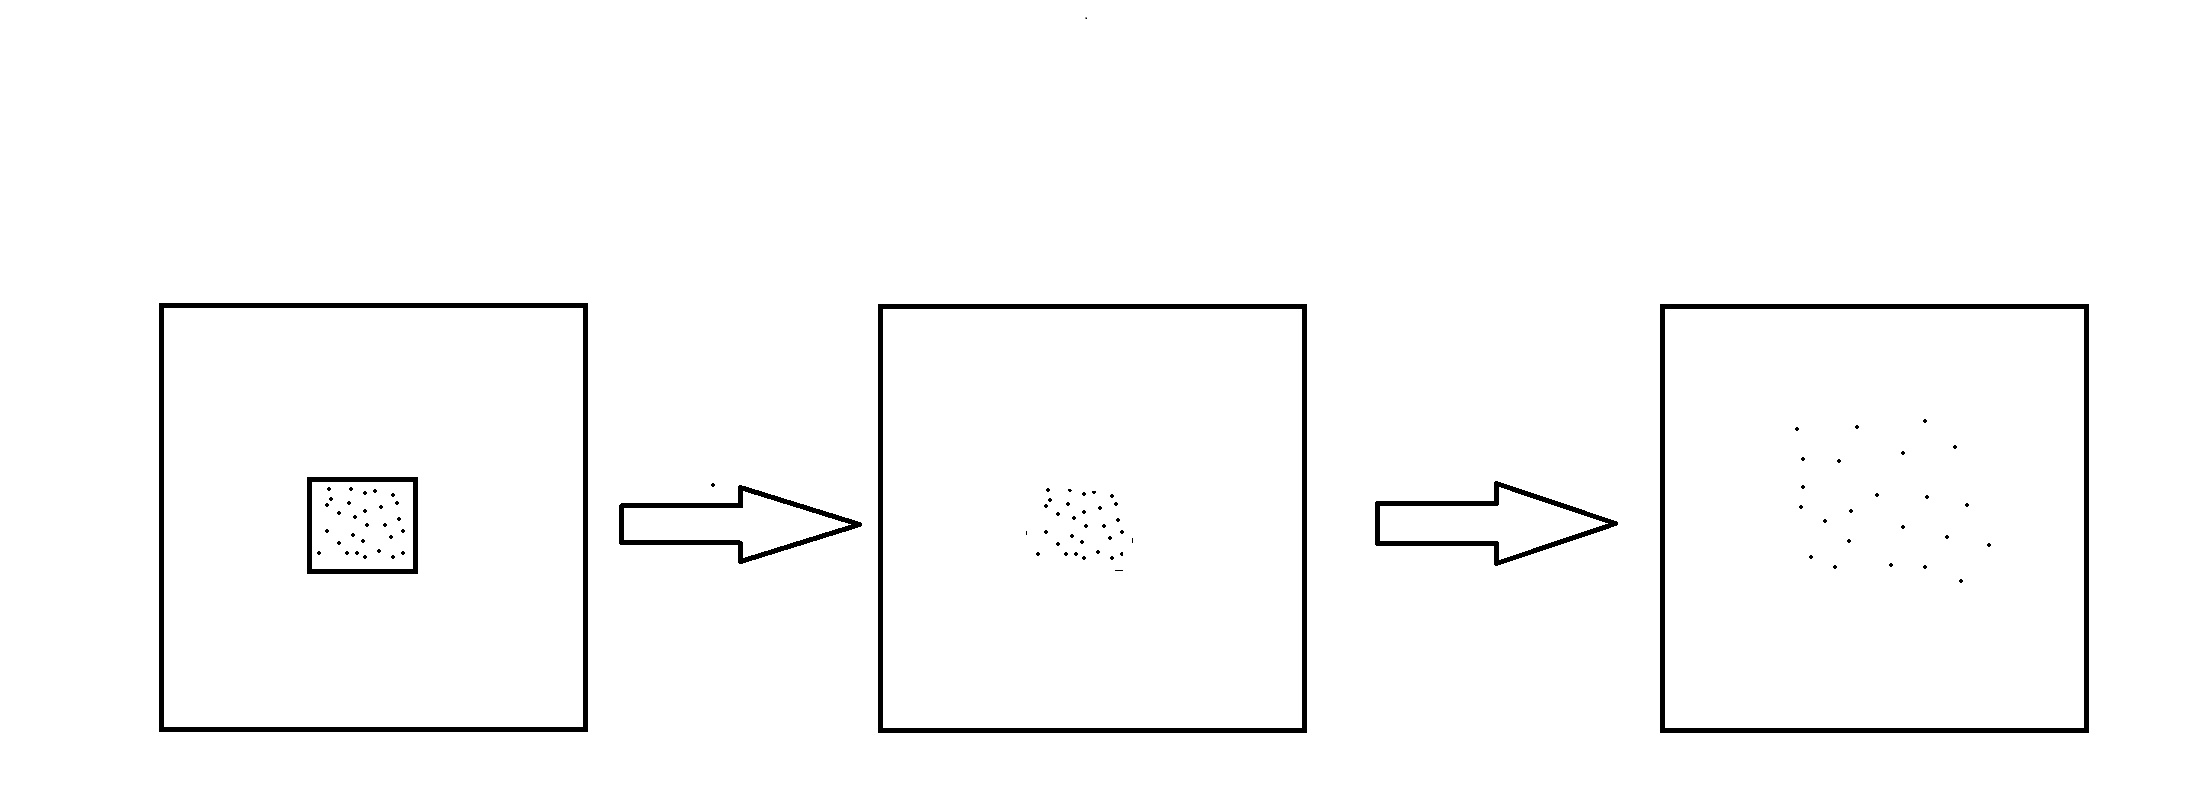
\includegraphics[width=10cm]{nishimura/image/2017112201.png}
  \caption{インクの広がりのイメージ図}
\end{figure}

「一度広がったインクは広がる状態の前に自然に戻ることはない」と断言したが、本当にそうなのかと疑問に思う人もいるだろう。それは不規則に運動するインクの分子が偶然、元の位置に戻ってくることがあってもいいのではないかという疑問だと思う。結論から言うと、そうなる確率がとても小さいので起こりにくいというのが答えだ。それを示すために気体分子を新しく例に挙げて考えてみよう。\par
大きな箱の中に小さな箱が入っており、小さな箱の中にN個の気体分子が入っているとしよう。\\

大きな箱と小さな箱の体積比が$9:1$だとすると、$1$個の分子が小さな箱に入る確率は$1/10$だ。よって、$N$個の分子なら、一つ一つの分子が独立関係なので、$N$個の分子が全て小さな箱に入る確率$P$は
\begin{align}
 P=\left (\frac{1}{10}\right)^N
\end{align}
になる。$1\mathrm{mol}$の気体で考えると$N=6.02×10^{23}$個とすれば、$P$がとても小さいことが分かる。経験的に部屋の空気がいきなり自然に部屋の隅に偏らないのはそうなる確率が低いからだ。もし、そんなことが起きれば部屋の中の人が窒息してしまう。\par
また、例に挙げたインクや気体分子が広がるというのは、広がる前よりも無秩序になったと言い換えることができる。まとめると自然に起こる変化はいつも無秩序さが増して、その変化は不可逆である。\newpage

%
\section{無秩序さとエントロピー}
\subsection{エントロピーとは}
セクション\ref{sec:hukagyaku}で紹介した無秩序さについて、それを量的に捉えることを考える(エネルギーみたいに)。そこで登場するのがエントロピーだ。\par

体積Vの箱を用意し、それを体積の$V_0$微小領域に分割する(図\ref{fig:V})。分子がどれに入るかで分子の状態を表すとする。セクション\ref{sec:hukagyaku}と同様に考えると、
\begin{align}
  \mathrm{1個の分子がとりうる状態の数} = \frac{V}{V_0}\\
	\mathrm{2個の分子がとりうる状態の数} = \left(\frac{V}{V_0}\right)^2\\
\mathrm{N個の分子がとりうる状態の数} = \left(\frac{V}{V_0}\right)^N \label{eq:W-N}
\end{align}
となる。$N$個の分子がとりうる状態の数を$W$とすると(\ref{eq:W-N})式より

\begin{align}
  \mathrm{W} =\left(\frac{V}{V_0}\right)^N  \label{itiyonn}
\end{align}
\begin{figure}[H]
  \centering
  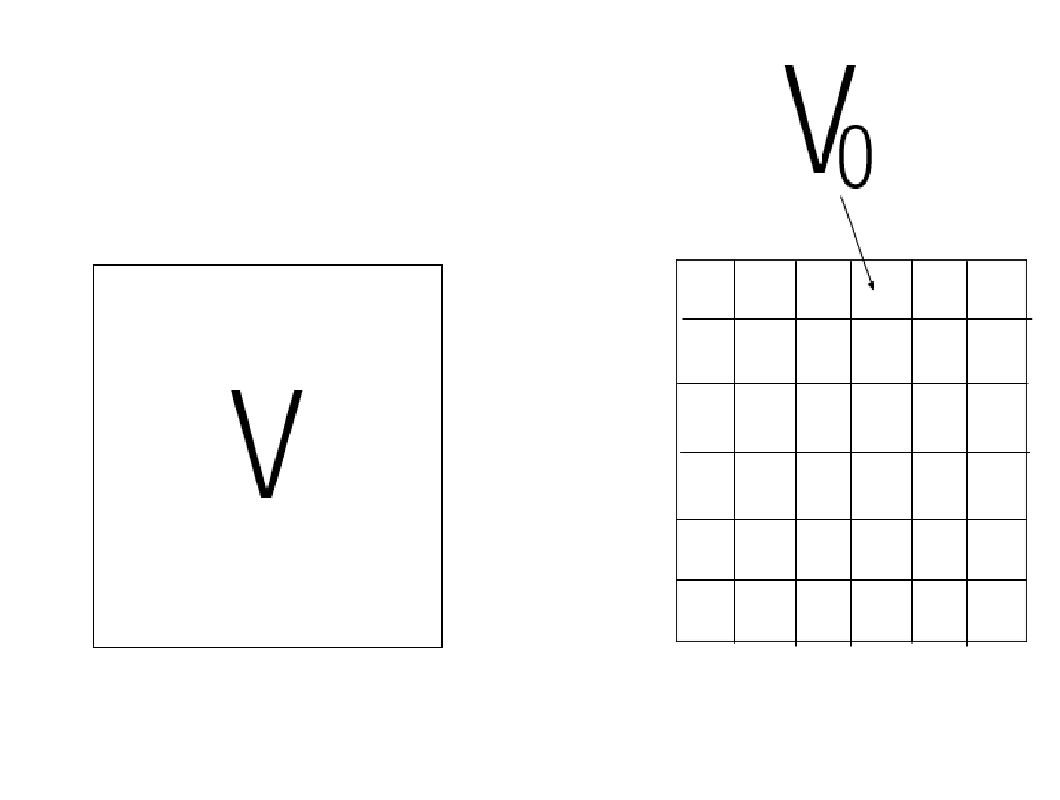
\includegraphics[width=10cm]{nishimura/image/2017112202.png}
  \caption{体積$V$の箱と体積$V_0$の微小領域}
  \label{fig:V}
\end{figure}
ここで、体積が$V_1$から$V_2$に変わった時の$W$の変化について考える。
\begin{align}
  \frac{W_2}{W_1}=\left(\frac{V_2}{V_1}\right)^N
\end{align}
無秩序さを表す量はエネルギーのように個数$N$に比例してほしい。だから、対数を用いてエントロピー$S$を定義する
\begin{align}
  S=k_B \ln{W} \label{eq:itiroku}
\end{align}
ここで、$k_B$はボルツマン定数と呼ばれていてボルツマン定数は$k_B=1.381×10^{23}[J\ K^{-1}]$である。\par
(\ref{eq:itiroku})の$W$に(\ref{itiyonn})を代入すると、
\begin{align}
  S=N k_B \ln{V}+定数  \label{snkb}
\end{align}
体積が$V_1$から$V_2$に変わったときのエントロピーが$S_1$から$S_2$になるとすれば、エントロピーの変化量は
\begin{align}
 \Delta S=S_2-S_1=N k_B \ln{\frac{V_2}{V_1}}  \label{itihati}
\end{align}
(\ref{itihati})より$V_2\textgreater V_1$なら$S_2\textgreater S_1$だから、体積が増加したらエントロピーが増加することがわかる。
\subsection{気体分子の速度の無秩序さ}
$速度空間で分子が分布している領域の体積\equiv \Omega$\\
$気体がその分子の速度についてとりうる状態の数\equiv W$\\
とすると、
\begin{align}
  W\propto \Omega^N   \label{itikyuu}
\end{align}
よって、エントロピーSは
\begin{align}
  S= N k_B \ln{\Omega}+定数
\end{align}
速度空間における、半径を$\overline{v}$,分子一個当たりのエネルギーを$\frac{E}{N}$とすると、
\begin{align}
  \frac{1}{2}m\overline{v}^2 &\simeq \frac{E}{N}\\
  \Rightarrow \overline{v} &\simeq \left(\frac{2E}{mN}\right)^{1/2}
\end{align}
したがって、領域の体積は
\begin{align}
  \Omega \simeq \frac{4}{3}\pi \overline{v}^3 \simeq \frac{4}{3}\pi \left(\frac{2E}{mN}\right)^{3/2}  \label{iisa}
\end{align}
これを(\ref{itikyuu})式に代入して、エネルギーに依存する部分だけを書くと、
\begin{align}
  W\propto \left(\frac{E}{N}\right)^{3N/2}   \label{iiyo}
\end{align}
(\ref{eq:itiroku})式に(\ref{iiyo})式を代入すると
\begin{align}
  S=\frac{3}{2}N k_B \ln{E}+定数   \label{iiro}
\end{align}
(\ref{iiro})式よりエネルギーが増加すると、エントロピーも増加することが分かる。
\section{気体の断熱変化}
断熱変化とは...エントロピーの増加をゼロとみなしていいような変化。\par
(\ref{iiro})式に気体の内部エネルギーと温度の関係
\begin{align}
  E=\frac{3}{2}N k_B \ln{T}
\end{align}
を代入すると、
\begin{align}
  S=\frac{3}{2}N k_B \ln{T} +定数   \label{itinana}
\end{align}
気体の断熱膨張を考えると、エントロピーは(\ref{snkb})式に従って増加するが、温度変化(減少)するので、(\ref{itinana})式に従って減少する。よって、
\begin{align}
  E&=Nk_B\ln{V}+\frac{3}{2}N k_B \ln{T}+定数\\
    &=Nk_B\ln VT^{3/2}+ 定数   \label{iiku}
\end{align}
$\Delta S=0の時にVT^{3/2}=一定となる。$

\section{秩序から無秩序へ}
統計力学によると温度$T$の環境の中に置かれた物体がエネルギー$E$の状態にある確率$P(E)$は
\begin{align}
  P(E)\propto\exp{(-E/{k_BT})}    \label{inio}
\end{align}
エネルギー$E$のミクロな状態の数$W$とすると、$W$個の状態一つ一つが(\ref{iiku})式によって実現する。\par
よって、マクロな状態にある確率$P'(E)$は
\begin{align}
   P'(E)\propto W\exp{(-E/{k_BT}) }   \label{inii}
\end{align}
(\ref{eq:itiroku})のエントロピーの定義より、
\begin{align}
   W=\exp{(S/k_B)}   \label{inini}
\end{align}
(\ref{inini})式を(\ref{inii})式に代入すると,
\begin{align}
   P'(E)\propto \exp{(-(E-TS)/{k_BT})}   \label{ijisa}
\end{align}
自由エネルギー$F$を
\begin{align}
   F\equiv E-TS    \label{Fteigi}
\end{align}
と定義する。\par
確率$P'(E)$が最大になるためには、$F$が最小になればよいので

\begin{align}
  \frac{dF}{dE}=1-T\frac{dS}{dE}=0\\
	\Rightarrow \frac{dS}{dE}=\frac{1}{T} \label{inigo}
\end{align}
温度一定で物体に$\Delta Q$の熱を加えたとすると、内部エネルギーは$\Delta E=\Delta Q$だけ増加する。\\
これを(\ref{inigo})式に使うと、エントロピーの変化量$\Delta S$は
\begin{align*}
  \Delta S=\frac{\Delta Q}{T}
\end{align*}
温度$T$と温度$\Delta Q$でエントロピーをあらわせた。
\section{熱力学の法則}
{\bf 熱力学の第一法則(エネルギー保存則)}\par
\begin{align}
   Q=\Delta U +W
\end{align}
(加えた熱を$Q$、内部エネルギーの変化量を$\Delta U$、気体が外にした仕事を$W$とした。)\par
{\bf 熱力学の第二法則(エントロピー増大測)}
\begin{align}
   \Delta S\geqq 0
\end{align}
($\Delta S$はエントロピーの増加量で等号成立は可逆過程の時)\par
{\bf 熱力学の第三法則}\\
\begin{align}
   `絶対零度では完全な秩序状態が実現する'
\end{align}
\ 第一法則と第二法則は経験則でわかる。系全体のエネルギーが保存するのは当たり前で、自然に起こる変化は乱雑になっていくことから、この二つは理解できる。\par
第三法則は何か難しいことを言っているように見えるが、ここまでの話から理解することができる。まず、温度が低いほどエントロピーは小さい((\ref{iiro})式より)。(\ref{Fteigi})式で$T=0$の時、$F=E$になる。絶対零度でエネルギーが最小なので、$F$も最小になる。$F$が最小ということは、マクロな状態にある確率$P'(E)$が最大で、確率は$1$になり、とりうる状態の数は一つに決まる。つまり、$T=0$で$W=1$。エントロピーの定義を考えると、$T→0$なら$S→0$になる。




%参考文献
%thebibliographyは使わないでください。\chapterになっちゃう!
\section*{参考文献}
\begin{enumerate}
  \item 長岡洋介、1997年、極低温の世界-超伝導への道-、岩波書店
 \item Sinshu Univ.Physical Chemistry Lab.Adsorption Group、定数について、「\url{science.shinshu-u.ac.jp/~tiiyama/?page_id=1564}」
\end{enumerate}





%
